\documentclass{/home/janmebows/Documents/LatexTemplates/myassignment}
\title{Topic C Assignment 2}

\begin{document}

\maketitle

\begin{enumerate}
    \item 
    \begin{enumerate}
        \item %find first 3 terms v_0(t) + \epsilon v_1(t) + \epsilon^2 v_2(t), \epsilon \to 0
        Let 
        \[v(t) = v_0(t) + \epsilon v_1(t) + \epsilon^2 v_2(t) + \bigo(\epsilon^3) \]
        \[\frac{dv}{dt} = \frac{dv_0(t)}{dt} + \epsilon \frac{dv_1(t)}{dt} + \epsilon^2\frac{dv_2(t)}{dt} + \bigo(\epsilon^3)\]
        \begin{align*}
            &\frac{dv}{dt} + \epsilon v^2 + t = 0\\
            &\frac{dv_0(t)}{dt} + \epsilon \frac{dv_1(t)}{dt} + \epsilon^2\frac{dv_2(t)}{dt} +\bigo(\epsilon^3) + \epsilon(v_0(t) + \epsilon v_1(t) + \epsilon^2 v_2(t) + \bigo(\epsilon^3))^2 + t = 0
        \end{align*}
        Subject to the IC:
        \begin{align*}
            &v(0) = 0\\
            \implies &v_0(0) + \epsilon v_1(0) + \epsilon^2 v_2(0) + \bigo(\epsilon^3) = 0
        \end{align*}
        \[\frac{dv_0(t)}{dt} + \epsilon \frac{dv_1(t)}{dt} + \epsilon^2\frac{dv_2(t)}{dt} + \epsilon \left(v_0(t) + \epsilon v_1(t) \right)^2 +t + \bigo(\epsilon) = 0\]
        \[\frac{dv_0(t)}{dt} + \epsilon \frac{dv_1(t)}{dt} + \epsilon^2\frac{dv_2(t)}{dt} + \epsilon v_0(t)^2 + \epsilon^2 v_0(t)v_1(t) +t + \bigo(\epsilon^3) = 0\]
        Collecting powers of epsilon gives the set of equations:
        \begin{align*}
            \frac{dv_0(t)}{dt} + t &= 0, \quad v_0(0) = 0\\
            \frac{dv_1(t)}{dt} + v_0(t)^2 &= 0, \quad v_1(0) = 0 \\
            \frac{dv_2(t)}{dt} + v_0(t)v_1(t) &= 0, \quad v_2(0) = 0
        \end{align*}
        Solve $v_0$:
        \begin{align*}
            \frac{dv_0(t)}{dt} + t &= 0, \quad v_0(0) = 0\\
            v_0(t) &= \int -t dt\\
            &= -\frac{t^2}{2} + C\\
            v_0(0) = 0 \implies v_0(t) &= -\frac{t^2}{2}
        \end{align*}
        Now solve $v_1$:
        \begin{align*}
            \frac{dv_1(t)}{dt} + v_0(t)^2 &= 0, \quad v_1(0) = 0 \\
            v_1(t) &= \int -\frac{t^4}{4} dt\\
            &= -\frac{t^5}{20} + C\\
            v_1(0) = 0 \implies v_1(t) &= -\frac{t^5}{20}
        \end{align*}
        Lastly, solve $v_2$:
        \begin{align*}
            \frac{dv_2(t)}{dt} + v_0(t)v_1(t) &= 0, \quad v_2(0) = 0\\
            v_2(t) &= \int -\left(\frac{t^5}{20}\frac{t^2}{2}\right)dt\\
            &= \int -\left(\frac{t^7}{40}\right)dt\\
            &= - \frac{t^8}{320} +C\\
            v_2(0) = 0 \implies v_2(t) &= -\frac{t^8}{320}
        \end{align*}
        Thus the expansion of $v(t)$ is
        \begin{align*}
            v_t(t) &= v_0(t) + \epsilon v_1(t) + \epsilon^2 v_2(t) + \bigo(\epsilon^3)\\
            &= -\frac{t^2}{2} - \epsilon \frac{t^5}{20} - \epsilon^2 \frac{t^8}{320} + \bigo(\epsilon^3)\\
            \therefore v_t(t) &\sim -\frac{t^2}{2} - \epsilon \frac{t^5}{20} - \epsilon^2 \frac{t^8}{320}
        \end{align*}
        as $\epsilon \to 0$
        \item%find where it is no longer valid
        The range of times $t$ for which this expansion is valid are those such that
        \[v_0(t) \gg \epsilon v_1(t) \gg \epsilon^2 v_2\]
        I.e. $t$ such that
        \[\frac{t^2}{2} \gg \epsilon \frac{t^5}{20} \gg -\epsilon^2 \frac{t^8}{320}\]
        For $v_0$, $\epsilon v_1$:
        
        $\epsilon v_1 \ll v_0$ if:
        \[\lim_{\epsilon \to 0} \frac{\epsilon v_1(t)}{v_0(t)} =0\]
        So find $t$ such that this limit doesn't converge to $0$
        \begin{align*}
            \lim_{\epsilon \to 0} \frac{\epsilon v_1(t)}{v_0(t)} &=\lim_{\epsilon \to 0} \frac{-\epsilon \frac{t^5}{20}}{-\frac{t^2}{2}}\\
            &= \lim_{\epsilon\to 0} \epsilon \frac{t^3}{10}\\
            &= \frac1{10 }\lim_{\epsilon\to 0 } \epsilon t^3
        \end{align*}
        This limit converges to $0$ if $t^3$ is $\bigo(\epsilon^{-1}$, i.e. we require
        \[0 \leq t \leq \bigo(\epsilon^{-1/3})\]
        
        For $\epsilon v_1$, $\epsilon^2 v_2$
        \begin{align*}
            \lim_{\epsilon\to 0} \frac{\epsilon^2 v_2}{\epsilon v_1} &= \lim_{\epsilon\to 0} \frac{\epsilon \frac{t^8}{320}}{\frac{t^5}{20}}\\
            &= \lim_{\epsilon\to 0} \frac{\epsilon t^3}{16}
        \end{align*}
        And hence this converges if $t^3 \leq \bigo(\epsilon)$, and as before
        \[0 \leq t \leq \bigo(\epsilon^{-1/3})\]


        I.e. we require $t \leq \bigo(\epsilon^{-1/3})$ for the asymptotic ordering to hold
    \end{enumerate}













    \item 
    \begin{enumerate}
        \item %first 3 terms in an expansion
        Want to find 
        \[\psi = \psi_0 + \epsilon \psi_1 + \epsilon^2 \psi_2\]
        Which satisfies
        \[\nabla^2 \psi = -1\]

        Use a taylor series to expand around the boundary condition
        \begin{align*}
            \psi_{y=\pm(1+\epsilon\cos kx)} = \psi_{y=\pm1} \pm \epsilon\cos kx\dd\psi y_{y=\pm1} + \frac12\epsilon^2\cos^2kx \ddn\psi y2_{y=\pm1} =0
        \end{align*}




        % \[\psi_{y=\pm1(1+\epsilon\cos kx)} = \sum_{n=0}^\infty \ddn{\psi}yn\frac{(\pm(1+\epsilon \cos kx)^n}{n!}\]
        % \begin{align*}
        % \psi_{y=\pm(1+\epsilon\cos kx)} &= \psi_{y=0} \pm(1+\epsilon\cos kx) \dd{\psi}y_{y=0} + \frac12(1+\epsilon\cos kx)^2 \ddn \psi y 2_{y=0} \pm \frac1{6}(1+\epsilon\cos kx)^3\ddn\psi y3\\
        %     =\psi_{y=0} &\pm(1+\epsilon\cos kx) \dd{\psi}y_{y=0} + \frac12(1+2\epsilon\cos kx + \epsilon^2\cos^2 kx) \ddn \psi y 2_{y=0} \\
        %     &\pm \frac16(1+2\epsilon\cos kx + \epsilon^2\cos^2 kx+ \epsilon\cos kx+2\epsilon^2\cos^2 kx + \epsilon^3\cos^3 kx)\ddn\psi y3\\
        %     =\psi \pm &\dd\psi y + \frac12\ddn\psi y2 \pm \frac16\ddn\psi y3 + \epsilon\cos kx\left(\pm\dd\psi y + \ddn \psi y2 \pm \frac12 \ddn\psi y3\right)+ \epsilon^2\cos^2kx\left(\frac12\ddn\psi y2 \pm \frac12\ddn\psi y3\right)
        % \end{align*}
        % At $y=0$
        
        % Subbing this into the boundary condition, and collect powers of $\epsilon$:
        % \begin{align*}
        %     \bigo(1): \ 0= &\psi_0 \pm \dd{\psi_0}y + \frac12\ddn{\psi_0}{y}2\\
        %     \bigo(\epsilon): 0= \ &\psi_1 \pm \dd{\psi_1}y+ \frac12\ddn{\psi_1}y2 + \cos kx(\pm \dd{\psi_0}{y} + \ddn{\psi_0}y2 \pm \frac12\ddn{\psi_0}y3)\\
        %     \bigo(\epsilon^2): \ 0= & \psi_2 \pm \dd{\psi_2}y+ \frac12\ddn{\psi_2}y2 + \cos kx(\pm \dd{\psi_1}{y} + \ddn{\psi_1}y2 \pm \frac12\ddn{\psi_1}y3) + \cos^2 kx \left(\frac12\ddn{\psi_0}y2 \pm \frac12 \ddn{\psi_0}y3\right)\\
        % \end{align*}
        % Where all of these are for $y=0$.

        For zeroth order:
        Since the flow is unperturbed in the $x$ direction, assume
        \[ \psi_0(x,y) = a + by + cy^2\]
        Using the boundary condition:
        \begin{align*}
            a \pm b + c = 0
        \end{align*}
        Hence $b=0$, and $a=-c$.
        Using the flow description:
        \begin{align*}
            \nabla^2\psi_0=2c&=-1\\
            \implies c = -\frac12\\
            \implies b = \frac12
        \end{align*}
        Hence
        \[\boxed{\psi_0 = \frac12\left(1 - y^2\right)}\]

        \textbf{Now first order}, $\bigo(\epsilon)$:
        \begin{align*}
            \nabla^2 \psi_1 = 0
        \end{align*}
        With boundary:
        \begin{align*}
            \psi_{1} \pm \cos kx \dd{\psi_0}y = 0, \quad y=\pm1\\
            \psi_{1} \pm \cos kx (-y) = 0, \quad y=\pm 1
        \end{align*}

        % With boundary condition
        % \begin{align*}
        %     0&=\psi_1 \pm \dd{\psi_1}y+ \frac12\ddn{\psi_1}y2 + \cos kx(\pm \dd{\psi_0}{y} + \ddn{\psi_0}y2 \pm \frac12\ddn{\psi_0}y3)\\
        %     &= \psi_1 \pm \dd{\psi_1}y + \frac{1}{2}\ddn{\psi_1}y2 + \cos kx\left(0 - \frac14\right)\\
        %     &= \psi_1 \pm \dd{\psi_1}y + \frac{1}{2}\ddn{\psi_1}y2 \mp\frac14 \cos kx\\
        % \end{align*}

        
        Let $\psi_1 = f(x)g(y)$
        \begin{align*}
            f''g + g''f = 0\\
            \frac{f''}f =- \frac{g''}g = \lambda
        \end{align*}
        \begin{itemize}
            \item $\lambda = 0$
            \[f'' = 0\]
            \[f = ax + b\]
            \[g = cy + d\]
            This cannot satisfy the boundaries.

            \item $\lambda=\mu^2 > 0$ 
            \[f'' = \mu^2 f\]
            %\[f = ae^{\mu x} + be^{-\mu x}\]
            \[f = a\cosh(\mu x) + b \sinh(\mu x)\]
            And for $g$
            \[g'' = - \mu^2 g\]
            \[g = c\sin(\mu y) + d \cos(\mu y)\]

            \begin{align*}
                f(0) = a = a\cosh(\mu 2\pi/k) + b\sinh(\mu 2\pi /k)
            \end{align*}
            True if $\mu =k$
            \[\psi_1 = (a\cosh kx + b\sinh kx)(c\sin ky + d\cos ky)\]
            \begin{align*}
            \psi_{1} \pm \cos kx (-y) = 0, \quad y=\pm 1\\
            (a\cosh kx + b\sinh kx)(c\sin(\pm k) + d\cos(\pm k)) \pm \cos kx (-y) = 0
            \end{align*}
            Which gives trivial solutions.


            \item $\lambda =\mu^2 < 0$
            \[f = a\sin(\mu x) + b\cos(\mu x)\]
            \[g = c\sinh(\mu y) + d\cosh(\mu y)\]
            \begin{align*}
                f(0) =a\sin(0) + b\cos(0) =  b = f(2\pi/k)\\
                f(2\pi/k)= a\sin(2\mu \pi/k) + b\cos(2\mu \pi/k) 
            \end{align*}
            This gives $\mu = k$

            Using the boundary condition:
            \begin{align*}
                (a\sin(k x) + b\cos(k x))(c\sinh(\pm k) + d\cosh(\pm k)) \pm (\mp)\cos kx = 0\\
                (a\sin(k x) + b\cos(k x))(\pm c\sinh(k) + d\cosh(k)) =\cos kx \\
                (a\tan(k x) + b)(\pm c\sinh(k) + d\cosh(k)) =1\\
                a\tan kx + b = \frac{1}{\pm c\sinh k + d\cosh k}
            \end{align*}
            Clearly $a=c=0$ for non-trivial solutions
            \[b = \frac{1}{d\cosh(k)}\]
            Hence
            \[\boxed{\psi_1 = \frac{\cos kx \cosh ky}{\cosh k}}\]

        \end{itemize}

        For $\psi_2$:
        \begin{align*}
        \nabla^2 \psi_2= 0
        \end{align*}

        Boundary condition:
        \begin{align*}
            \psi_2 \pm \cos kx \dd{\psi_1}y + \cos^2kx \ddn{\psi_0} y2 = 0, \ y=\pm 1\\
            \psi_{2,y=\pm1} \pm \cos kx \frac{k \cos kx \sinh(\pm k)}{\cosh k} - \cos^2 kx=0\\
            \psi_{2,y=\pm1} +(k\tanh(k) - 1)\cos^2 kx=0\\
            \implies \psi_{2,y=\pm1} = (1 - k\tanh(k))\cos^2 kx
        \end{align*}
        And $\psi_2(0,y) = \psi_2 (2\pi/k,y)$, 

        $\psi_2$ will have form:
        \[\psi_2 = g(y) (1 - k\tanh(k))\cos^2 kx \]
        Where $h(\pm1) = 0$

        \begin{align*}
            \nabla^2 \psi_2 = g''(y) (1 - k\tanh(k))\cos^2 kx + g(y)(1-k\tanh(k))2k^2(\sin^2 kx - \cos^2 kx)\\
            g''(y) (1 - k\tanh(k))\cos^2 kx - 4k^2g(y)(1-k\tanh(k))\cos^2 kx=0\\
            g''(y) - 4k^2g(y)=0\\
            \frac{g''}g = 4k^2\\
            \implies g = a_*e^{2k y} + b_*e^{-2ky}\\
            \implies g = a\cosh 2ky + b \sinh 2ky
        \end{align*}
        Require $g(\pm1) = 1$
        \begin{align*}
            g(\pm1) =a\cosh (\pm2k) + b \sinh (\pm2k)=1\\
             a\cosh(2k) \pm b \sinh(2k) = 1\\
             b=0,\quad a = \frac{1}{\cosh 2k}
        \end{align*}
        Hence
        \[\boxed{\psi_2 =  \frac{(1 - k\tanh(k))}{\cosh2k} \cos^2 kx \cosh 2ky}\]

        Therefore:
        \[\boxed{\psi =\frac12(1-y^2) + \epsilon\left(\frac{\cos kx \cosh ky}{\cosh k}\right) + \epsilon^2\left(\frac{(1 - k\tanh(k))\cos^2 kx \cosh 2ky}{\cosh2k} \right) }\]
        Figure~\ref{fig::q2psi} shows the contour of $\psi$ for $k=0.6$ and $\epsilon=0.1$. The
        \begin{figure}[h]
        \centering
        \label{fig::q2psi}
        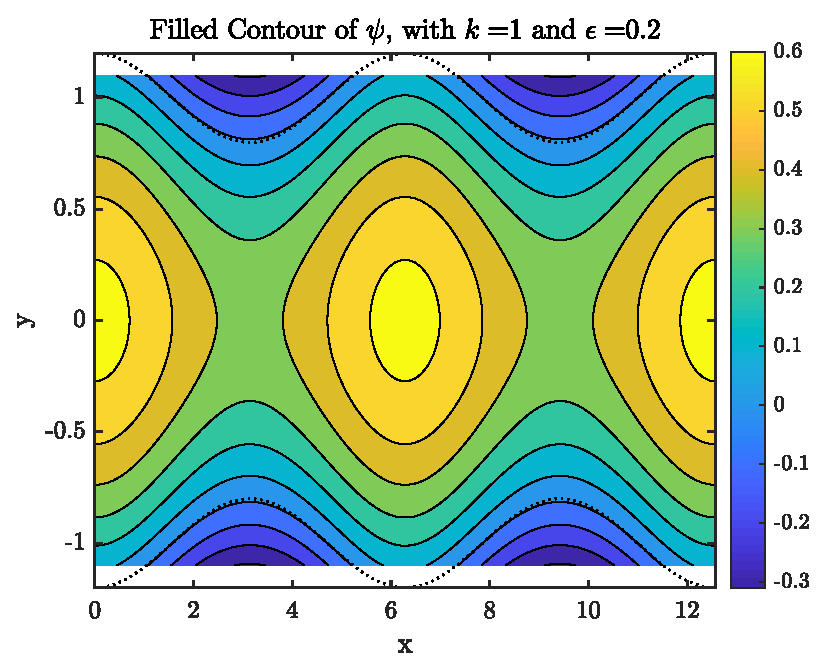
\includegraphics[]{TopicCA2Q2a}
        \caption{Contour of $\psi$ against a given $k$ and $\epsilon$ The dotted line represents the boundary conditions, at $y= \pm(1+\epsilon\cos kx)$ }
        \end{figure}
        \item %plot streamlines
        %using the obtained streamfunction, get streamlines
        Streamlines will be
        \begin{align*}
            u &= \dd\psi y\\
            &=-y + \epsilon k\left(\frac{\cos kx \sinh ky}{\cosh k}\right) + \epsilon^2 2k\left(\frac{(1 - k\tanh(k))\cos^2 kx \sinh 2ky}{\cosh2k} \right)
        \end{align*}
        \begin{align*}
            v &= -\dd\psi x\\
            &=\epsilon k\left(\frac{\sin kx\cosh ky}{\cosh k}\right) + \epsilon^2 2k\left(\frac{(1 - k\tanh(k))\sin kx\cos kx \sinh 2ky}{\cosh2k}\right)
        \end{align*}
        
        \begin{figure}[h]
            \centering
            \label{fig::q2stream}
            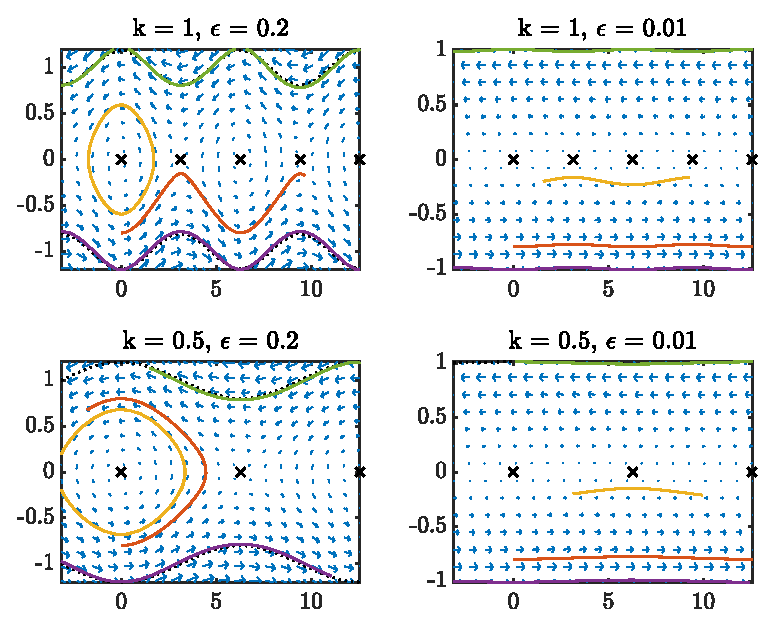
\includegraphics[]{TopicCA2Q2b}
            \caption{Streamline plots for various $k$ and $\epsilon$ with some example paths. $\times$ marks stagnant points in the flow, the purple and green lines are the flows along the negative and positive boundaries respectively, yellow and red are example paths}
        \end{figure}

        Figure~\ref{fig::q2stream} shows the plots of the streamlines. The vertically the plots show a change in $k$, while across is a change in $\epsilon$. Note when $\epsilon$ gets quite large, closed loops can form (the yellow paths for the two left plots).
        \item %comment on validity
        If $k=\frac{n\pi}{2}$ for $n=1,3,5,\hdots$ there can be issues, Since the $\epsilon$ and $\epsilon^2$ terms become infinite. 
        Since the boundary is 
        \[y = \pm (1+\epsilon \cos kx)\]
        If $\epsilon >= 1$ we will have regions of the flow where the boundaries will overlap I.e. $-h(x;\epsilon) >= h(x;\epsilon)$

        The assumption that the channel is infinitely long is also necessary. The formulae used assumed incompressible flow, so we expect the flux of flow to be low when the gap between the boundaries is largest, i.e. for $x = 2nk\pi$ for integer $n$. Similarly we expect it to be the largest when $x = \frac{\pi}2 + nk\pi$.

        The solution is also questionable as there are these stagnation points which the flow circulates around. 
        
    \end{enumerate}













    \item %%%%BIG HINT APPARENTLY THEY WILL GROW AND EXPLODE KINDA LIKE THE VIDEO
    %%Note that everything with a 1 pertains to the above flow. I.e. the one with the region y > \epsilon h(x,t)
    \begin{enumerate}
        \item %expand to get the conditions around y=0 
        %this question wants me to expand out the kinermatic conditions
        %and the bernoulli condition.
        I will use $h := h(x,t)$ for shorthand
        Linearise the conditions about the unperturbed interface, $y=0$. Using a taylor series:
        \begin{align*}
            \dd\phi y\pipe_{y=\epsilon h} &= \dd\phi y\pipe_{y=0} + \epsilon h\ddn \phi y2 \pipe_{y=0} + \bigo(\epsilon^2)\\
            \dd\phi x\pipe_{y=\epsilon h} &= \dd\phi x \pipe_{y=0} + \epsilon h \frac{\partial^2 \phi}{\partial x \partial y}\pipe_{y=0} + \bigo(\epsilon^2)\\
            \dd\phi t\pipe_{y=\epsilon h} &= \dd\phi t \pipe_{y=0} + \epsilon h \frac{\partial^2 \phi}{\partial t \partial y}\pipe_{y=0} + \bigo(\epsilon^2)
        \end{align*}
        Since we are only considering powers up to $\epsilon$ (neglecting $\epsilon^2$) I will drop all $\epsilon^2$ (and higher) terms. 

        \textbf{Kinematic Conditions}
        \begin{align*}
            \dd{\phi}y &= \epsilon \left(\dd ht + \dd{\phi}x \dd hx \right), \quad y=\epsilon h(x,t)\\
            \dd\phi y + \epsilon h \ddn \phi y2  &= \epsilon\left(\dd h t + \dd hx \left(\dd\phi x + \epsilon h \frac{\partial^2 \phi}{\partial x \partial y}\right)\right),\quad y=0
        \end{align*}
        Which is now on $y=0$, for both $\phi_1$ and $\phi_2$.\\
        \textbf{Bernoulli Condition}
        \begin{align*}
            \rho_1 \left(\dd{\phi_1}{t} - \frac12 c_1^2 + \frac12 |\nabla \phi_1|^2 + gy \right) = \rho_2 \left(\dd{\phi_2}{t} - \frac12 c_2^2 + \frac12 |\nabla \phi_2|^2 + gy \right) , \quad y=\epsilon h(x,t)\\
            \rho_1\left(\dd{\phi_1} t\pipe_{y=0} + \epsilon h\dd{\phi_1}{y\partial t} \pipe_{y=0} -\frac12 c_1^2 + \frac12 |\nabla\phi_{1_{y=0}}|^2 + \epsilon g h\right)\\
            =\rho_2\left(\dd{\phi_2} t\pipe_{y=0} + \epsilon h\dd{\phi_2}{y\partial t} \pipe_{y=0}-\frac12 c_2^2 + \frac12 |\nabla \phi_{2_{y=0}}|^2 + \epsilon gh\right)\\
        \end{align*}
        On $y=0$.

        Where all of these conditions are true up to $\bigo(\epsilon^2)$
        \item %introduce perturbation series for $\phi_1, \phi_2$
        %solve for the first term of each, 
        %and write down the problems for the second terms
        Introducing
        \begin{align*}
            \phi_1(x,y,t) = \phi_{10}(x,y,t) + \epsilon\phi_{11}(x,y,t) + \bigo(\epsilon^2)\\
            \phi_2(x,y,t) = \phi_{20}(x,y,t) + \epsilon\phi_{21}(x,y,t) + \bigo(\epsilon^2)\\
        \end{align*}
        Now collect powers for all the conditions:

        \textbf{Kinematic condition:}
        \begin{align*}
            \bigo(1):\ &\dd{\phi_{\#0}}y = 0\\
            \bigo(\epsilon):\ &\dd{\phi_{\#1}}y + h\ddn{\phi_{\#0}}y2 = \dd ht + \dd hx\left(\dd{\phi_{\#0}}x\right)
        \end{align*}
        \textbf{Bernoulli condition:}
        \begin{align*}
            \bigo(1):\ &\rho_1\left(\dd{\phi_{10}}t - \frac12 c_1^2 + \frac12\left(\left(\dd{\phi_{10}}y\right)^2 + \left(\dd{\phi_{10}}x\right)^2 + \dd{\psi_{10}}x \dd{\psi_{10}}y \right)\right)\\
            &=\rho_2\left(\dd{\phi_{20}}t - \frac12 c_2^2 + \frac12\left(\left(\dd{\phi_{20}}y\right)^2 + \left(\dd{\phi_{20}}x\right)^2 + \dd{\psi_{20}}x \dd{\psi_{20}}y \right)\right)\\
        \end{align*}
        I will write the $\bigo(\epsilon)$ version below.

        The unperterbed problem is described by:
        \[\nabla^2\phi_{10} = 0, \quad y >0\]
        \[\nabla^2\phi_{20} = 0, \quad y >0\]
        With kinematic conditions:
        \[\dd{\phi_{10}} y  =  0, \quad y=0\]
        \[\dd{\phi_{20}} y  =  0, \quad y=0\]
        The flow equation reduces to
        \[\ddn{\phi_{\#0}}x2 = 0\]
        Which gives
        \[\phi_{\#0} = A_{\#} x + B_{\#}\]
        And using the condition far awayfrom the interface, it gives
        \[\phi_{10} = c_1 x\]
        \[\phi_{20} = c_2 x\]

        To first power of $\epsilon$, the problem becomes:


        \textbf{Flow description}
        \begin{align*}
            \nabla^2 \phi_{\#1} = 0
        \end{align*}
        For $\phi_1$ with $y > 0$, and for $\phi_2$ around $y < 0$

        \textbf{Kinematic Condition}
        \begin{align*}
            \dd{\phi_{\#1}}y + h\ddn{\phi_{\#0}}y2 = \dd ht + \dd hx\left(\dd{\phi_{\#0}}x\right)\\
            \dd{\phi_{\#1}}y = \dd ht + \dd hx\left(\dd{\phi_{\#0}}x\right)
        \end{align*}
        


        
        \textbf{Bernoulli Condition}
        \begin{align*}
        &\rho_1\Big(\dd{\phi_{11}}t + h\frac{\partial \phi_{10}}{\partial y\partial t} + \frac12(|\nabla \phi_1|^2+ gh\Big)\\
            &=\rho_2\Big(\dd{\phi_{21}}t + h\frac{\partial \phi_{20}}{\partial y\partial t} + \frac12 |\nabla\phi_2|^2+ gh\Big)\\\\
        \end{align*}
        On $y=0$, extracting the $\bigo(\epsilon)$ part of $|\nabla\phi_{\#}|^2$.

        With the far condition that
        \[\phi_{11} = 0 , \quad y \to \infty\]
        \[\phi_{21} = 0 , \quad y \to -\infty\]



        \item %use separation of variables to obtain the 2nd terms using the problem found before
        Assume
         \[h(x,t) = ae^{i(kx-\omega t)}\]

        Since it is Laplaces' equation, we can assume that $\phi_{\#1}$ has form:
        \[\phi_{\#1} = f(y) e^{i(kx-\omega t)}\]
        \begin{align*}
            \nabla^2\phi_{\#1} = (-k^2 f + f'')e^{i(kx-\omega t}) = 0\\
            -k^2 f + f'' = 0\\
            f''/f = k^2\\
            \implies f_{\#} = be^{k_{\#}y}
        \end{align*}
        To satisfy the far field conditions:
        \begin{align*}
            \phi_{11} = 0 ,\quad y\to \infty\\
            \implies e^{k_{1}\infty} = 0\\
            \phi_{21} = 0 ,\quad y\to -\infty\\
            \implies e^{-k_{2}\infty} = 0\\
        \end{align*}
        And so $k_1 = -k$ and $k_2 = k$.
        Hence
        \[\phi_{11} =b_1e^{-ky} e^{i(kx-\omega t)},\quad \phi_{21} =b_2e^{ky} e^{i(kx-\omega t)}\]

        Now using the kinematic condition(s)
        \begin{align*}
            \dd{\phi_{11}}y &= \dd ht + \dd hx\left(\dd{\phi_{\#0}}x\right), \quad y=0\\
            -kb_{1} e^{-k0}e^{i(kx-\omega t)}  &= -i\omega a e^{i(kx-\omega t)} + iac_{1}e^{i(kx-\omega t)}\\
            -kb_{1} &= -i\omega a + iac_{1} k \\
            b_{1} &= \frac{i\omega a - iac_{1} k}{k}\\
            &= (-ai) \frac{-\omega + c_{1}k }{|k|}
        \end{align*}

        \begin{align*}
            \dd{\phi_{21}}y = \dd ht + \dd hx\left(\dd{\phi_{\#0}}x\right)\\
            kb_{2} e^{i(kx-\omega t)}  &= -i\omega a e^{i(kx-\omega t)} + iac_{2}ke^{i(kx-\omega t)}\\
            kb_{2} &= -i\omega a + iac_{2} k \\
            b_{2} &= \frac{-i\omega a + iac_{2} k}{k}\\
            &= (ai) \frac{-\omega + c_{2}k }{k}\\
        \end{align*}
        Hence
        \[\phi_{11} = (-ai)\frac{-\omega  + c_{1} k}{k}e^{-ky} e^{i(kx-\omega t)},\quad \phi_{21} = (ai)\frac{-\omega  + c_{2} k}{k}e^{ky} e^{i(kx-\omega t)}\]
                




        \item %substitute into the boundary conditions to get \omega
        Calculate (at $\bigo(\epsilon)$):
        \[|\nabla \phi|^2,\quad y=0 \]
        Expanding $|\nabla \phi|^2_{\epsilon}$, where the subscript $\epsilon$ is the order
        \begin{align*}
            |\nabla \phi_{1}|^2_{\epsilon} &= |\nabla \phi_{10} + \epsilon\nabla \phi_{11}|^2_{\epsilon}\quad (y=0)\\
            &=\pipe c_1 + \epsilon ik(-ai)\frac{-\omega  + c_{1} k}{k}e^{-ky} e^{i(kx-\omega t)} -\epsilon  k(-ai)\frac{-\omega  + c_{1} k}{k}e^{-ky} e^{i(kx-\omega t)}\pipe ^2_{\epsilon}\\
            &=\pipe c_1 + \epsilon ka\frac{-\omega  + c_{1} k}{k} e^{i(kx-\omega t)} + \epsilon kai\frac{-\omega  + c_{1} k}{k}e^{i(kx-\omega t)}\pipe ^2_{\epsilon}\\
            &= \left(c_1 + \epsilon ka\frac{-\omega  + c_{1} k}{k} e^{i(kx-\omega t)}\right)^2 + \left(\epsilon ka\frac{-\omega  + c_{1} k}{k}e^{i(kx-\omega t)}\right)^2_{\epsilon}\\
            &= 2c_1ka\frac{-\omega  + c_{1} k}{k} e^{i(kx-\omega t)}\\
            &= i2kc_1 \phi_{11,y=0}
        \end{align*}
        And for $\phi_2$:
        \begin{align*}
            |\nabla \phi_{2}|^2_{\epsilon} &= |\nabla \phi_{20} + \nabla \epsilon\phi_{21}|^2_{\epsilon}\quad (y=0)\\
            &=\pipe c_2 + \epsilon ik(ai)\frac{-\omega  + c_{2} k}{k}e^{-ky} e^{i(kx-\omega t)} -\epsilon  k(ai)\frac{-\omega  + c_{2} k}{k}e^{-ky} e^{i(kx-\omega t)}\pipe ^2_{\epsilon}\\
            &=\pipe c_2 - \epsilon ka\frac{-\omega  + c_{2} k}{k} e^{i(kx-\omega t)} - \epsilon kai\frac{-\omega  + c_{2} k}{k}e^{i(kx-\omega t)}\pipe ^2_{\epsilon}\\
            &= \left(c_2 - \epsilon ka\frac{-\omega  + c_{1} k}{k} e^{i(kx-\omega t)}\right)^2 + \left(\epsilon ka\frac{-\omega  + c_{2} k}{k}e^{i(kx-\omega t)}\right)^2_{\epsilon}\\
            &= -2c_2ka\frac{-\omega  + c_{2} k}{k} e^{i(kx-\omega t)}\\
            &= i2kc_2\phi_{21,y=0}
        \end{align*}



        Now using the bernoulli condition:
        \begin{align*}
            &\rho_1\left(\dd{\phi_{11}}t + \frac12\left(|\nabla\phi_1|^2_{\epsilon} \right) + gh\right) =\rho_2\left(\dd{\phi_{21}}t + \frac12\left(|\nabla\phi_2|^2_{\epsilon}\right) + gh\right)\\  
            &\rho_1\left(\dd{\phi_{11}}t + \frac12\left(i2kc_1 \phi_{11} \right) + gh\right) =\rho_2\left(\dd{\phi_{21}}t + \frac12\left(i2kc_2 \phi_{21}\right) + gh\right)\\\\  
            &\rho_1\left(-i\omega(-ai)\frac{-\omega  + c_{1} k}{k} e^{i(kx-\omega t)} + ikc_1(-ai)\frac{-\omega  + c_{1} k}{k} e^{i(kx-\omega t)} + gae^{i(kx-\omega t)}\right) \\
            &=\rho_2\left(-i\omega(ai)\frac{-\omega  + c_{2} k}{k}e^{i(kx-\omega t)} + ikc_2 (ai)\frac{-\omega  + c_{2} k}{k}e^{i(kx-\omega t)} + gae^{i(kx-\omega t)}\right)\\\\   
            &\rho_1\left(-\omega a\frac{-\omega  + c_{1} k}{k} + kc_1a\frac{-\omega  + c_{1} k}{k}  + ga\right) =\rho_2\left(\omega a\frac{-\omega  + c_{2} k}{k}- kc_2a\frac{-\omega  + c_{2} k}{k}+ ga\right)\\  
            &\rho_1\left(\frac{a\omega^2  - c_{1} k a \omega-\omega kc_1a  + c_{1}^2k^2 a }{k}  + ga\right) =\rho_2\left(\frac{-a\omega^2   + c_{2} ka\omega +kc_2a\omega  - c_{2}^2 k^2a}{k}+ ga\right)\\  
            &\rho_1\left(\omega^2  - 2c_{1} k \omega  + c_{1}^2k^2 + gk\right) + \rho_2\left(\omega^2 - 2c_{2} k\omega + c_{2}^2 k^2- gk\right)=0\\
            & (\rho_1+\rho_2)\omega^2  - (\rho_1c_1+\rho_2c_2)2 k  \omega  + (\rho_1c_{1}^2+\rho_2c_2^2)k^2 + (\rho_1-\rho_2)gk=0\\
        \end{align*}

        Which is a quadratic in $\omega$
        \begin{align*}
            \omega &=\frac{2k(\rho_1c_1+\rho_2c_2) \pm \sqrt{4k^2(\rho_1c_1+\rho_2c_2)^2 -4(\rho_1+\rho_2)((\rho_1c_1^2+\rho_2c_2^2)k^2+(\rho_1-\rho_2)gk)}}{2(\rho_1+\rho_2)}
        \end{align*}
        Cleaning the square root:
        \begin{align*}
            \Delta \omega &= 4k^2(\rho_1c_1+\rho_2c_2)^2 -4(\rho_1+\rho_2)((\rho_1c_1^2+\rho_2c_2^2)k^2+(\rho_1-\rho_2)gk)\\
            &=4k^2(\rho_1^2c_1^2 + \rho_2^2c_2^2 + 2\rho_1\rho_2c_1c_2) \\&- 4(\rho_1^2c_1^2k^2 + \rho_2^2c_2^2k^2 + \rho_1\rho_2c_2^2k^2 + \rho_2\rho_1c_1^2k^2 + \rho_1^2gk + \rho_2^2gk )\\\\
            &=4k\left(2k\rho_1\rho_2c_1c_2 - \rho_1\rho_2c_2^2k -\rho_1\rho_2c_1^2k -\rho_1^2g -\rho_2^2g\right)
        \end{align*}
        \item %use \omega to determine stability of the interface in terms of c_1,c_2,\rho_1,\rho_2,k
        Noting that $\rho_1,\rho_2 > 0$ is a physical constraint.
        There will be imaginary part (and hence solutions will be unstable) if
        \begin{align*}
             4k\left(2k\rho_1\rho_2c_1c_2 - \rho_1\rho_2c_2^2k -\rho_1\rho_2c_1^2k -\rho_1^2g -\rho_2^2g\right) < 0\\
             2k\rho_1\rho_2c_1c_2 - \rho_1\rho_2c_2^2k -\rho_1\rho_2c_1^2k < gk(\rho_1^2 +\rho_2^2)\\
            \rho_1\rho_2k^2\left(2c_1c_2 - c_2^2 - c_1^2\right) < gk(\rho_1^2+\rho_2^2)\\
            \frac{\rho_1\rho_2}{\rho_1^2 + \rho_2^2}\left(c_1+c_2\right)^2 > -\frac gk \\
            \text{positive thing} > -\frac{1}{k}
         \end{align*} 
         So positive $k$ (and small negative values) will give unstable solutions, which will blow up. Otherwise, the conditions will be purely oscillatory and will not die out/blow up.

        %interpret the physical significance of the result (presumably some values will explode, some will decay)
    \end{enumerate}
\end{enumerate}


\section*{Matlab Code}
\lstinputlisting{AppTopicCA2.m}

\clearpage
\includepdf[pages=1-]{PA_2019_A2.pdf}

\end{document}
